\subsection{Encrypted-Age-Verification}
\label{sub:encrypted_age_verification}

\subsubsection{Funktionsbeschreibung}
Der Use Case Encrypted Age Verification löst das Problem, das Alter einer Person serverseitig zu prüfen, ohne dass der Server den tatsächlichen Alterswert jemals im Klartext zu Gesicht bekommt. Das Ergebnis der Prüfung (volljährig: ja/nein) wird ebenfalls verschlüsselt zurückgegeben - der Server kennt weder Eingabe noch Ausgabe. \par
Das Alter wird bereits auf dem Client mit dem ClientKey verschlüsselt und ausschließlich in verschlüsselter Form an das Backend übertragen. 
Das Backend führt die Altersüberprüfung mittels Fully Homomorphic Encryption (TFHE) durch, ohne den zugrunde liegenden Alterswert entschlüsseln zu können. 
Die Entschlüsselung des Ergebnisses ist ausschließlich durch den Besitzer des ClientKeys möglich.

\textbf{Akteure}:
\begin{itemize}
    \item Client: Generiert das TFHE-Schlüsselpaar, verschlüsselt das Alter mit dem \verb|ClientKey|, sendet \verb|encrypted_age| und \verb|server_key| an den Server, empfängt das verschlüsselte Ergebnis und entschlüsselt es lokal. Der Client besitzt den \verb|ClientKey| und ist der einzige Akteur, der das Ergebnis entschlüsseln kann.
    \item Backend (Server): Empfängt \verb|encrypted_age| und \verb|CompressedServerKey|, setzt den ServerKey, führt die homomorphe Altersüberprüfung (\verb|age_check|) durch und gibt das verschlüsselte Ergebnis (\verb|FheBool|) zurück. Der Server sieht zu keinem Zeitpunkt das Alter oder das Ergebnis im Klartext.
\end{itemize}

\textbf{Lebenszyklus einer Session}

\subsubsection{Phase 1 -- Session-Setup (einmalig)}

\begin{enumerate}
  \item Client generiert \texttt{ClientKey} und \texttt{CompressedServerKey} lokal. Das Alter wird als \texttt{FheInt8} mit dem \texttt{ClientKey} verschl\"usselt.
  \item Client sendet \texttt{POST /session} mit dem \texttt{CompressedServerKey} (${\sim}80\,\text{MB}$) als JSON-Body.
  \item Server dekomprimiert den Key einmalig (\texttt{CompressedServerKey::decompress()}), speichert den \texttt{ServerKey} im \texttt{AppState} und gibt eine \texttt{session\_id} (UUID) zur\"uck.
\end{enumerate}

\subsubsection{Phase 2 -- Verifikation}

\begin{enumerate}[start=4]
  \item Client sendet \texttt{POST /verify/\{session\_id\}} mit ausschlie\ss{}lich \texttt{encrypted\_age} im Body.
  \item Server liest den gecachten \texttt{ServerKey} aus dem \texttt{AppState}, f\"uhrt \texttt{age\_check} aus (\texttt{enc\_age.gt(17) \& enc\_age.ge(0)}) und gibt das verschl\"usselte \texttt{FheBool}-Ergebnis zur\"uck.
  \item Client entschl\"usselt das \texttt{FheBool} mit dem \texttt{ClientKey} und erh\"alt das boolesche Ergebnis.
\end{enumerate}

\subsubsection{Phase 3 -- Cleanup}

\begin{enumerate}[start=7]
  \item Client sendet \texttt{DELETE /session/\{session\_id\}}, um die Session zu beenden und den serverseitigen RAM freizugeben.
\end{enumerate}

\textbf{Verhaltensdiagramm}:
\begin{figure}[H]
    \centering
    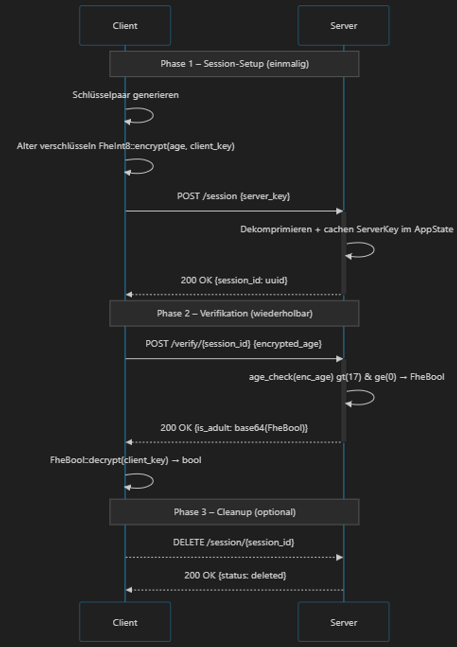
\includegraphics[width=\textwidth]{contents/media/UseCase2_Verhaltensdiagramm.png}
\end{figure}
    
\section{OpenAPI-Schnittstelle}

Der Service stellt eine session-basierte verschl\"usselte Verifikations-API bereit. Die OpenAPI-Definition wird automatisch generiert und ist unter \texttt{/openapi.json} sowie \texttt{/docs} (Swagger UI) erreichbar.

Im gesamten Service wird der ServerKey als \texttt{CompressedServerKey} \"ubertragen (bincode-serialisiert, base64-kodiert).

\subsection{POST /session}

L\"adt den \texttt{CompressedServerKey} einmalig hoch, dekomprimiert ihn und gibt eine \texttt{session\_id} zur\"uck.

\subsubsection*{Request}

\begin{lstlisting}
{
  "server_key": "string"
}
\end{lstlisting}

\subsubsection*{Response 200}

\begin{lstlisting}
{
  "session_id": "uuid"
}
\end{lstlisting}

\subsubsection*{Fehlercodes}

\begin{itemize}
  \item \textbf{400} -- Ung\"ultiges Base64 oder besch\"adigtes bincode in \texttt{server\_key}
\end{itemize}

\textbf{Body-Limit:} 2\,GiB (notwendig wegen der Gr\"o\ss{}e des \texttt{CompressedServerKey})

\subsection{POST /verify/\{session\_id\}}

F\"uhrt eine verschl\"usselte Altersverifikation durch.

\subsubsection*{Request}

\begin{lstlisting}
{
  "encrypted_age": "string"
}
\end{lstlisting}

\subsubsection*{Response 200}

\begin{lstlisting}
{
  "is_adult": "string"
}
\end{lstlisting}

\texttt{is\_adult} ist ein base64-kodierter, bincode-serialisierter \texttt{FheBool} -- \texttt{true}, wenn Alter $\geq 18$ und $\geq 0$.

\subsubsection*{Fehlercodes}

\begin{itemize}
  \item \textbf{400} -- Ung\"ultiges Base64 oder besch\"adigtes bincode in \texttt{encrypted\_age}
  \item \textbf{404} -- Session nicht gefunden
  \item \textbf{500} -- Serialisierungsfehler beim Kodieren des Ergebnisses
\end{itemize}

\subsection{DELETE /session/\{session\_id\}}

L\"oscht die Session und gibt den serverseitigen RAM frei.

\subsubsection*{Response 200}

\begin{lstlisting}
{
  "status": "deleted"
}
\end{lstlisting}

\subsubsection*{Fehlercodes}

\begin{itemize}
  \item \textbf{404} -- Session nicht gefunden
\end{itemize}

\subsubsection{Trust- und Threat-Model}
\begin{tabular}{||l|c|c|c||}
    \hline
    & \makecell{\textbf{Server}\\\textbf{klar}} & \makecell{\textbf{Server}\\\textbf{verschlüsselt}} & \makecell{\textbf{Nur Client}} \\
    \hline\hline
    Alter (numerischer Wert) & & X & \\
    \hline
    Ergebnis (volljährig: ja/nein) & & X & \\
    \hline
    ServerKey / CompressedServerKey & X & & X \\
    \hline
    ClientKey & & & X \\
    \hline
\end{tabular}

\textbf{Analyse: Beobachtbare Metadaten}:
TFHE schützt ausschließlich den Inhalt des Alters und des Ergebnisses. Für den Server bleiben weiterhin verschiedene Metadaten sichtbar:
\begin{itemize}
    \item Zeitpunkte und Häufigkeit der Anfragen
    \item IP-Adresse des anfragenden Clients
    \item Charakteristische Payload-Größe (~80 MB), die auf TFHE-Schlüsselübertragung schließen lässt
    \item Anzahl der Anfragen pro IP
\end{itemize}
Da \verb|age_check| eine datenunabhängige Berechnung ist (keine Branches auf verschlüsselten Werten), gibt es kein Timing-Side-Channel über die Rechendauer. Ein Server-Operator kann aus den Metadaten allenfalls Nutzungshäufigkeit ableiten, nicht jedoch das Alter einzelner Nutzer.

\textbf{Restvertrauen in den Server}:
Der Server kann zwar das Alter nicht entschlüsseln, muss jedoch weiterhin als korrekter Ausführer der Verifikationslogik vertrauenswürdig sein. Insbesondere wird angenommen, dass der Server:
\begin{itemize}
    \item \verb|age_check| korrekt und unverändert ausführt (kein Austausch gegen eine Funktion, die immer \verb|true| zurückgibt)
    \item Das korrekte \verb|FheBool|-Ergebnis zurücksendet und es nicht durch einen manipulierten Ciphertext ersetzt
    \item Den ServerKey nicht persistiert oder weitergibt
\end{itemize}
TFHE reduziert somit die Vertrauensabhängigkeit hinsichtlich der Inhaltsvertraulichkeit, ersetzt jedoch kein vollständig vertrauensloses Protokoll.

\textbf{Annahmen außerhalb von TFHE}:
Die Sicherheitsbetrachtung basiert auf folgenden Annahmen:
\begin{itemize}
    \item Die Kommunikation zwischen Client und Server erfolgt über TLS.
    \item Der Client führt Verschlüsselung und Entschlüsselung korrekt aus.
    \item Die verwendete TFHE-rs-Bibliothek wird als kryptographisch korrekt implementierte Black Box betrachtet.
    \item Es gibt keine Authentifizierung am Endpunkt: Jeder, der einen gültigen \verb|CompressedServerKey| besitzt, kann Anfragen stellen.
\end{itemize}
    
\textbf{Schutzversprechen}:
Durch den Einsatz von TFHE wird garantiert:
\begin{itemize}
    \item Der Server kann das Alter des Nutzers nicht im Klartext lesen.
    \item Der Server kann nicht feststellen, ob das Ergebnis \verb|true| oder \verb|false| ist.
    \item Das Alter wird ausschließlich verschlüsselt verarbeitet.
\end{itemize}
    
\textbf{Nicht garantiert werden}:
\begin{itemize}
    \item Schutz vor einem Server, der \verb|age_check| durch eine manipulierte Funktion ersetzt
    \item Schutz vor Traffic-Analyse (Payload-Größe, Timing)
    \item Authentizität des Clients (kein ZKP, dass der Client den ServerKey korrekt erzeugt hat)
\end{itemize}
    
\textbf{Konkret bedeutet das}: 
Der Server kennt nicht das Alter des Nutzers und kann nicht feststellen, ob das Ergebnis positiv oder negativ ausgefallen ist. Sichtbar bleiben ausschließlich Zeitpunkt, Herkunft und Häufigkeit der Anfragen.

\subsubsection{FHE-Designentscheidungen}
\textbf{Verwendete TFHE-rs-Typen}:
Für das Alter wird \verb|FheInt8| (vorzeichenbehaftetes 8-Bit-Integer, Wertebereich -128 bis 127) verwendet. Diese Wahl ergibt sich aus zwei Gründen:

Altersangaben in Jahren liegen typischerweise im Bereich 0-127, also weit innerhalb von \verb|i8|. \verb|FheUint8| wäre für den positiven Ast ausreichend, aber \verb|FheInt8| erlaubt es, negative Eingaben explizit als ungültig zu erkennen und abzufangen (s. \verb|is_positive-Check|). Zudem unterstützt \verb|FheInt8| \verb|gt| und \verb|ge| mit vorzeichenbehafteter Ganzzahlsemantik, was den Negativen-Grenzwert-Test (\verb|ge(0)|) korrekt macht.\par
Das Ergebnis ist ein \verb|FheBool| (verschlüsseltes Bit), was dem binären Charakter der Frage (volljährig: ja/nein) entspricht.

\textbf{Verwendete homomorphe Operationen}:
Der Server führt ausschließlich zwei Vergleiche und eine boolesche Verknüpfung aus. Andere homomorphe Operationen werden nicht benötigt, dadurch bleibt die serverseitige Auswertung auf die minimal nötige Anzahl FHE-Operationen beschränkt.\par
\begin{tabular}{||l|l||}
    \hline
    \textbf{Operation} & \textbf{Verwendung} \\
    \hline\hline
    \verb|FheInt8::gt| & \verb|enc_age > 17| $\rightarrow$ Alter $\geq$ 18 \\
    \hline
    \verb|FheInt8::ge| & \verb|enc_age > 0| $\rightarrow$ kein negativer Wert \\
    \hline
    \verb|FheBool::bitand| & Verknüpfung beider Bedingungen \\
    \hline
\end{tabular}

\textbf{Verworfene Alternativen}:
\verb|FheUint8| statt \verb|FheInt8| \par
Wäre für rein positive Eingaben ausreichend. Verworfen, weil damit keine sinnvolle Behandlung negativer Eingaben möglich ist - \verb|FheUint8| interpretiert \verb|-1| als \verb|255|, was den Negativen-Grenzwert-Test (\verb|age_check(-1) $\rightarrow$ false|) unmöglich machen würde. \par
Schwellwert als verschlüsselter Parameter \par
Denkbar wäre, den Grenzwert (18) ebenfalls als \verb|FheInt8| zu übergeben, um ihn serverseitig variabel zu halten. Verworfen, weil der Schwellwert in diesem Use Case keine schützenswerte Information ist und eine feste Konstante die Implementierung erheblich vereinfacht. \par
\verb|FheInt32| oder größere Typen \par
Größere Bitbreiten würden höhere Latenzen pro homomorpher Operation verursachen, ohne Mehrwert - Altersangaben benötigen keine mehr als 8 Bit.

\subsubsection{Komplexität der eigenen Algorithmen}
Da der Use Case ausschließlich aus einer festen Anzahl homomorpher Operationen auf einem einzelnen Ciphertext besteht, gibt es keine parametrisierten Eingabegrößen. Die Komplexität aller Funktionen ist konstant. \par
\begin{tabular}{||l|c|c||}
    \hline
    \textbf{Funktion} & \textbf{Zeitkomplexität} & \textbf{Platzkomplexität} \\
    \hline\hline
    \verb|descode_server_key| & O(1) & O(1) \\
    \hline
    \verb|decode_encrypted_age| & O(1) & O(1) \\
    \hline
    \verb|age_check| & O(1) & O(1) \\
    \hline
    \verb|encode_result| & O(1) & O(1) \\
    \hline
    \verb|verify_age| (gesamt) & O(1) & O(1) \\
    \hline
\end{tabular}\par
\textit{verify\_age - O(1), O(1)}\par
Die Funktion führt genau zwei Vergleiche (\verb|gt(17)|, \verb|ge(0)|) und eine AND-Verknüpfung (\verb|&|) auf einem \verb|FheInt8|-Wert durch. Alle drei sind Operationen fester Bitbreite (8 Bit) auf einem einzelnen Ciphertext - unabhängig von jeder Eingabegröße. Gemäß der Konvention, homomorphe Operationen als O(1) zu zählen, ist \verb|age_check| $\in$ O(1). \par
Die De- und Serialisierungsschritte (\verb|bincode|, \verb|base64|) operieren auf Byte-Arrays fester Länge (durch die TFHE-rs-Typen bestimmt) und sind ebenfalls O(1) bezüglich fachlicher Parameter.

\subsubsection{Performance-Messung}

\subsection{Mess-Setup \& Methodik}

Die Performance- und Stresstests wurden auf einem virtuellen KVM-Server von Netcup durchgef\"uhrt. Die Last wurde extern mittels k6 von einer lokalen Windows-Maschine \"uber das Internet injiziert.

Getestet wurde \texttt{POST /verify/\{session\_id\}} -- der rechenintensive Endpunkt. \texttt{POST /session} (einmaliger Setup) und \texttt{DELETE /session/\{id\}} (Cleanup) wurden nicht separat belastet, da sie nicht im kritischen Pfad der Verifikation liegen.
Die Gesamtlatenz setzt sich aus zwei Anteilen zusammen:
\begin{enumerate}
  \item Netzwerk\"ubertragung von \texttt{encrypted\_age} -- vernachl\"assigbar
  \item \texttt{age\_check()} -- zwei FHE-Vergleiche + AND-Verkn\"upfung auf dem gecachten \texttt{ServerKey}
\end{enumerate}

\textit{Test 1 -- Baseline (1 VU, 10 sequentielle Requests, session-basiert) (09.06.2026)}\par

\begin{tabular}{||l|l||}
    \hline
    \textbf{Metrik} & \textbf{Wert} \\
    \hline\hline
    p50 & 114,17 ms \\
    \hline
    p90 & 126,44 ms \\
    \hline
    p95 & 132,74 ms \\
    \hline
    Maximum & 176,31 ms \\
    \hline
    Fehlerrate & 0\% \\
    \hline 
    Durchsatz & ~1,47 req/s \\
    \hline
\end{tabular}

\textbf{Fazit:} Im session-basierten Modus entf\"allt der 80\,MB ServerKey-Transfer pro Request. 
Die eigentliche FHE-Operation (\texttt{age\_check}) dauert ${\sim}114\,\text{ms}$. p50 und p95 liegen eng beieinander (114\,ms vs.\ 133\,ms), was auf ein stabiles und vorhersehbares Systemverhalten hinweist.

\textit{Test 2 - Stresstest (ramping bis 10 VUs) (09.06.2026)}\par

\textbf{Methodik:} \texttt{setup()} baut alle 10 Sessions sequentiell auf, bevor der erste VU startet -- jede Session mit eigenem Schl\"usselpaar (\texttt{payload\_vu\{N\}\_sk.txt}, \texttt{payload\_vu\{N\}\_age.txt}). 
Erst wenn alle 10 Sessions bereit sind, beginnt die Lastphase. Jede VU greift ausschlie\ss{}lich auf ihre eigene Session zu (\texttt{\_\_VU \% 10}). 
Dadurch wird der ServerKey-Upload vollst\"andig aus der Latenzbetrachtung herausgehalten und 10 echte parallele Clients simuliert.

\begin{tabular}{||l|l||}
    \hline
    \textbf{Metrik} & \textbf{Wert}
    \hline\hline
    p50 & 114,06 ms \\
    \hline
    p90 & 126,27 ms \\
    \hline
    p95 & 130,43 ms \\
    \hline
    Maximum & 174,62 ms\\
    \hline
    Fehlerrate & 0 \% \\
    \hline
    Durchsatz & ~2,27 req/s \\
    \hline
\end{tabular}

\textit{Fazit von Test 2:}\par
Unter 10 parallelen Clients mit je eigenem Schl\"usselpaar und eigener Session bleibt die Verifikationslatenz nahezu identisch zur Baseline (p50: 114\,ms, p95: 130\,ms). 
Es treten keine Timeouts oder Fehler auf. Der \texttt{set\_server\_key}-Mutex wirkt sich nicht messbar aus, weil die FHE-Operation mit ${\sim}114\,\text{ms}$ kurz genug ist, dass parallele Requests keine nennenswerte Wartezeit verursachen.

\subsubsection{Limitationen}
\begin{itemize}
  \item Der \texttt{CompressedServerKey} (${\sim}80\,\text{MB}$) wird einmalig beim Session-Setup \"ubertragen und dekomprimiert gecacht. Folgende Verify-Requests enthalten nur noch \texttt{encrypted\_age}. Der gecachte \texttt{ServerKey} verbleibt im RAM des Servers, bis die Session per \texttt{DELETE /session/\{id\}} beendet wird -- es gibt keine automatische Ablaufzeit.

  \item Sessions haben keine Authentifizierung: Jeder, der eine \texttt{session\_id} kennt, kann Verify-Requests gegen diese Session stellen. In einer produktiven Umgebung m\"usste die Session an eine authentifizierte Identit\"at gebunden sein.

  \item Der Server pr\"uft nicht, ob ein \texttt{encrypted\_age}-Ciphertext bereits zuvor verwendet wurde. Ein Angreifer, der einen Ciphertext abf\"angt, kann ihn beliebig oft einreichen.

  \item Der Client \"ubergibt den \texttt{CompressedServerKey} selbst. Ein b\"osartiger Client k\"onnte einen manipulierten Key einreichen. In einer produktiven Umgebung m\"usste der ServerKey serverseitig fest hinterlegt sein.

  \item Der Client k\"onnte einen beliebigen \texttt{FheInt8}-Wert \"ubermitteln -- der Server kann nicht verifizieren, dass die verschl\"usselte Eingabe tats\"achlich ein Alter darstellt oder aus einer vertrauensw\"urdigen Quelle stammt.

  \item Maximal darstellbarer Alterswert ist 127 Jahre (\texttt{i8::MAX}). Dies ist f\"ur den Anwendungsfall ausreichend, aber die Wahl von \texttt{FheInt8} schlie\ss{}t gr\"o\ss{}ere Ganzzahlen strukturell aus.

  \item Es gibt keine Authentifizierung am Endpunkt. Jeder, der die API kennt, kann Anfragen stellen.
\end{itemize}